% ! TeX root = distributed-systems-final-report.tex
\section{Design}\label{design}

\subsection{Architecture}\label{arch:architecture}
The architecture is event-driven, revolving around a message oriented broker,
through a publish-subscribe mechanism. Under normal conditions, there's a
centralized controller to orchestrate traffic; however, each vehicle is also
provided with an autonomous and fully functioning logic (\textit{failsafe
mode}), in order to work even under network unavailability. Finally, a server,
subscribed to the same message broker, employs a REST API to serve the
simulation visualization to a client and to receive configuration commands.

This architecture type addresses many of the distributed systems features
discussed in the requirements.
\\
\\
First of all, the message based broker already provides naturally many forms of
\textbf{transparency} (\ref{req:distr_transparency}), since every node has to
only communicate with this, without having to know many details about the
others, not even their number (\textbf{scalability transparency}),
or having to share additional information with them.

Moreover, a broker, using a standard protocol for messages, makes it
straightforward, without any additional modification or configuration needed,
to: change the number of nodes (\textbf{scalability},
\ref{req:distr_scalability}); make modifications and improvements in a modular
way, to a single infrastructure component (evolvability, \ref{req:distr_evolv});
integrate different technologies, as long as they use the same communication
protocols (openness, \ref{req:distr_openness}).
\\
\\
Implementing an autonomous logic in each car was fundamental: it's the only way
to guarantee the required (requirement 6.1, \ref{req:req_fault}) fault tolerance
(\ref{req:distr_dependability}). In fact, even if the controller was perfectly
implemented to be always available, there can always be network issues, and a
car accident can't be accepted. Furthermore, one should also expect that some
vehicles may be completely unreachable: even if the controller has a way to
tackle this problem (refer to controller's behaviour, \ref{arch:behaviour}) by
receiving the cars in the local vision of each one, there can never be a
guarantee that it won't miss some, especially when there are only a few ones
responding and sharing data. Finally, even in normal conditions, a local logic,
without any network latency, constitutes an additional safety measure.
\\
\\
The web server doesn't have any other notable characteristics, since it's expected
to only be used by one, or few, people to visualize the simulation, thus without a
heavy load; even in a real life scenario, a similar solution may be used by just
a few system's maintainers for monitoring purposes.

\subsection{Infrastructure}\label{infrastructure}
The infrastructure follows simply from the architecture
(\ref{arch:architecture}), with components:

\begin{itemize}
  \item A car (replicated in multiple instances), comprising fictional sensors
  (sensing data), actuators (applying instructions) and their own logic.
  \item One controller.
  \item One messaage broker.
  \item One simulation service: subscribed to the same broker, it handles some
  tasks about the simulation itself, most of all detecting collisions between
  vehicles.
  \item One web-viewer.
\end{itemize}

The system uses Docker containerization to simulate a geographically distributed
environment. Each vehicle and each other component runs as an isolated process
in its own container, sharing only the broker's virtual network. So, every
communication happens through the broker, except the REST calls from the
simulation's viewer to the web server.

\begin{figure}
    \centering
    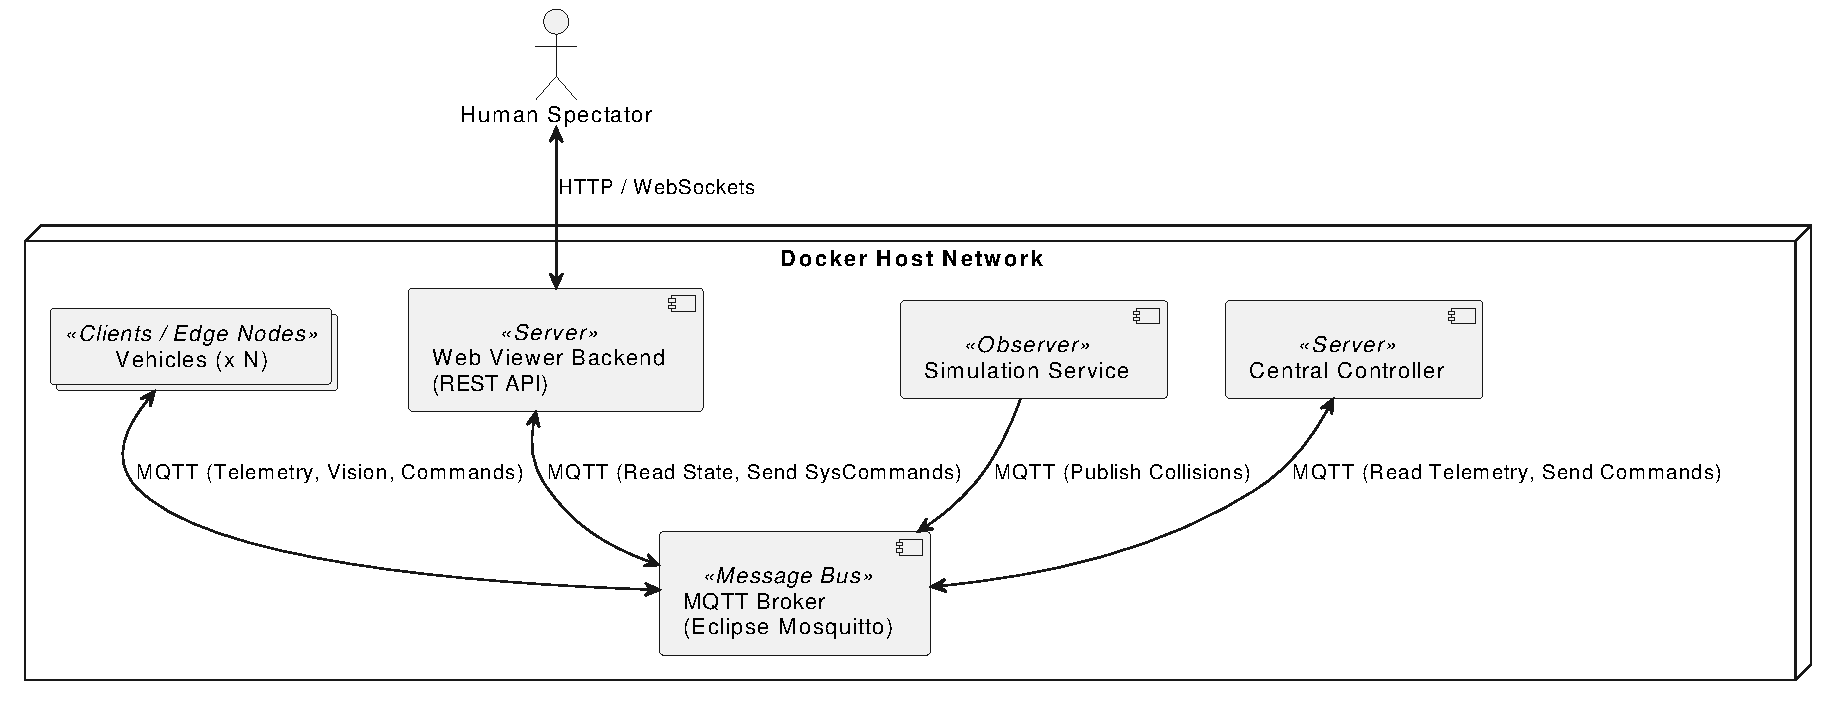
\includegraphics[width=\textwidth]{figures/component-diagram.pdf}
    \caption{The system's components and their communication paths.}
    \label{fig:component-diagram}
\end{figure}

\subsection{Modelling}\label{arch:modelling}
\textbf{Domain entities} are mostly constituted by the vehicles: the entity
defined as \textbf{vehicle position} only only contains spatial data (position
and speed); the \textbf{vehicle} entity contains the same spatial data plus some
additional information, such as acceleration, entry and exit road (to the
roundabout) and variables for displaying. Furthermore, for both vehicles and
positions, a \textbf{navigation state} is defined for convenience:
\textbf{approaching} when going towards the roundabout, \textbf{inside} when
driving around it, \textbf{exiting} when going away. Note that a \textbf{vehicle
position} reflects our model of what a car's local vision can perceive:
infra-red sensors would be able to quickly read another object's speed and
position.

In addition, there are entities for \textbf{controller commands} (issued to
vehicles) and \textbf{system commands} (configuration controls issued by the
viewer).

Each vehicle maintains:
\begin{itemize}
  \item its \textbf{local state}, as a \textbf{vehicle};
  \item a \textbf{vehicle position} for each car in its vision's range: a subset
  of the global state.
\end{itemize}

The controller maintains:
\begin{itemize}
  \item \texttt{active\_vehicles}: a dictionary of healthy \textbf{vehicles},
  transmitted directly by themselves;
  \item \texttt{precedence\_queue}: a queue to manage the order of arrival at the
  roundabout's entrance;
  \item \textbf{ghosts}: estimated \textbf{vehicle positions} of disconnected
  vehicles (reconstructed through the healthy ones' crowdsensing).
\end{itemize}

All data on the controller's node is kept up-to-date, i.e. old entries (older
than a certain threshold) are periodically purged, hence its never too different
from the real-time data, known by each vehicle alone.

All commands are exchanged over the network and used immediately, never stored.

Exchanged messages reflect the entities, and how they're perceived by each
component:
\begin{itemize}
  \item a periodical message for each healthy \textbf{vehicle}'s telemetry;
  \item a periodical message for each \textbf{vehicle} (even the disconnected
  ones): the controller doesn't utilize this, since this data wouldn't be
  available in real life, but the simulation does, in order to display the real
  state to the viewer;
  \item a periodical message for the objects in the local vision of each healthy
  vehicle;
  \item periodical messages for controller commands, indicating what
  acceleration the car should use;
  \item periodical controller messages to share its state (for debugging),
  containing its managed entities;
  \item messages for system commands, from the user to the web viewer (which
  will then communicate them to the correct recipient);
  \item messages for system commands, from the web viewer (after receiving one
  from the viewer), either towards individual vehicles or towards all at the
  same time in broadcast;
  \item messages for detected collisions, from the simulation component, to be
  displayed to the viewer;
\end{itemize}

Related to the messages, the main events can be identified as:
\begin{itemize}
  \item \textit{TelemetryUpdated}: a vehicle shares its kinematic state;
  \item \textit{VisionUpdated}: a vehicle shares the object detected through its
  local vision;
  \item \textit{CommandIssued}: the controller has evaluated the state and
  instructs a vehicle to accelerate or brake;
  \item \textit{CollisionDetected}: the simulation service identifies a car
  collision;
  \item \textit{SystemStateChanged}: the viewer user issues a system command;
  \item \textit{HeartbeatMissed/Timeout}: the timeout for lack of messages
  triggers a vehicle to transition to a failsafe state.
\end{itemize}

\begin{figure}
    \centering
    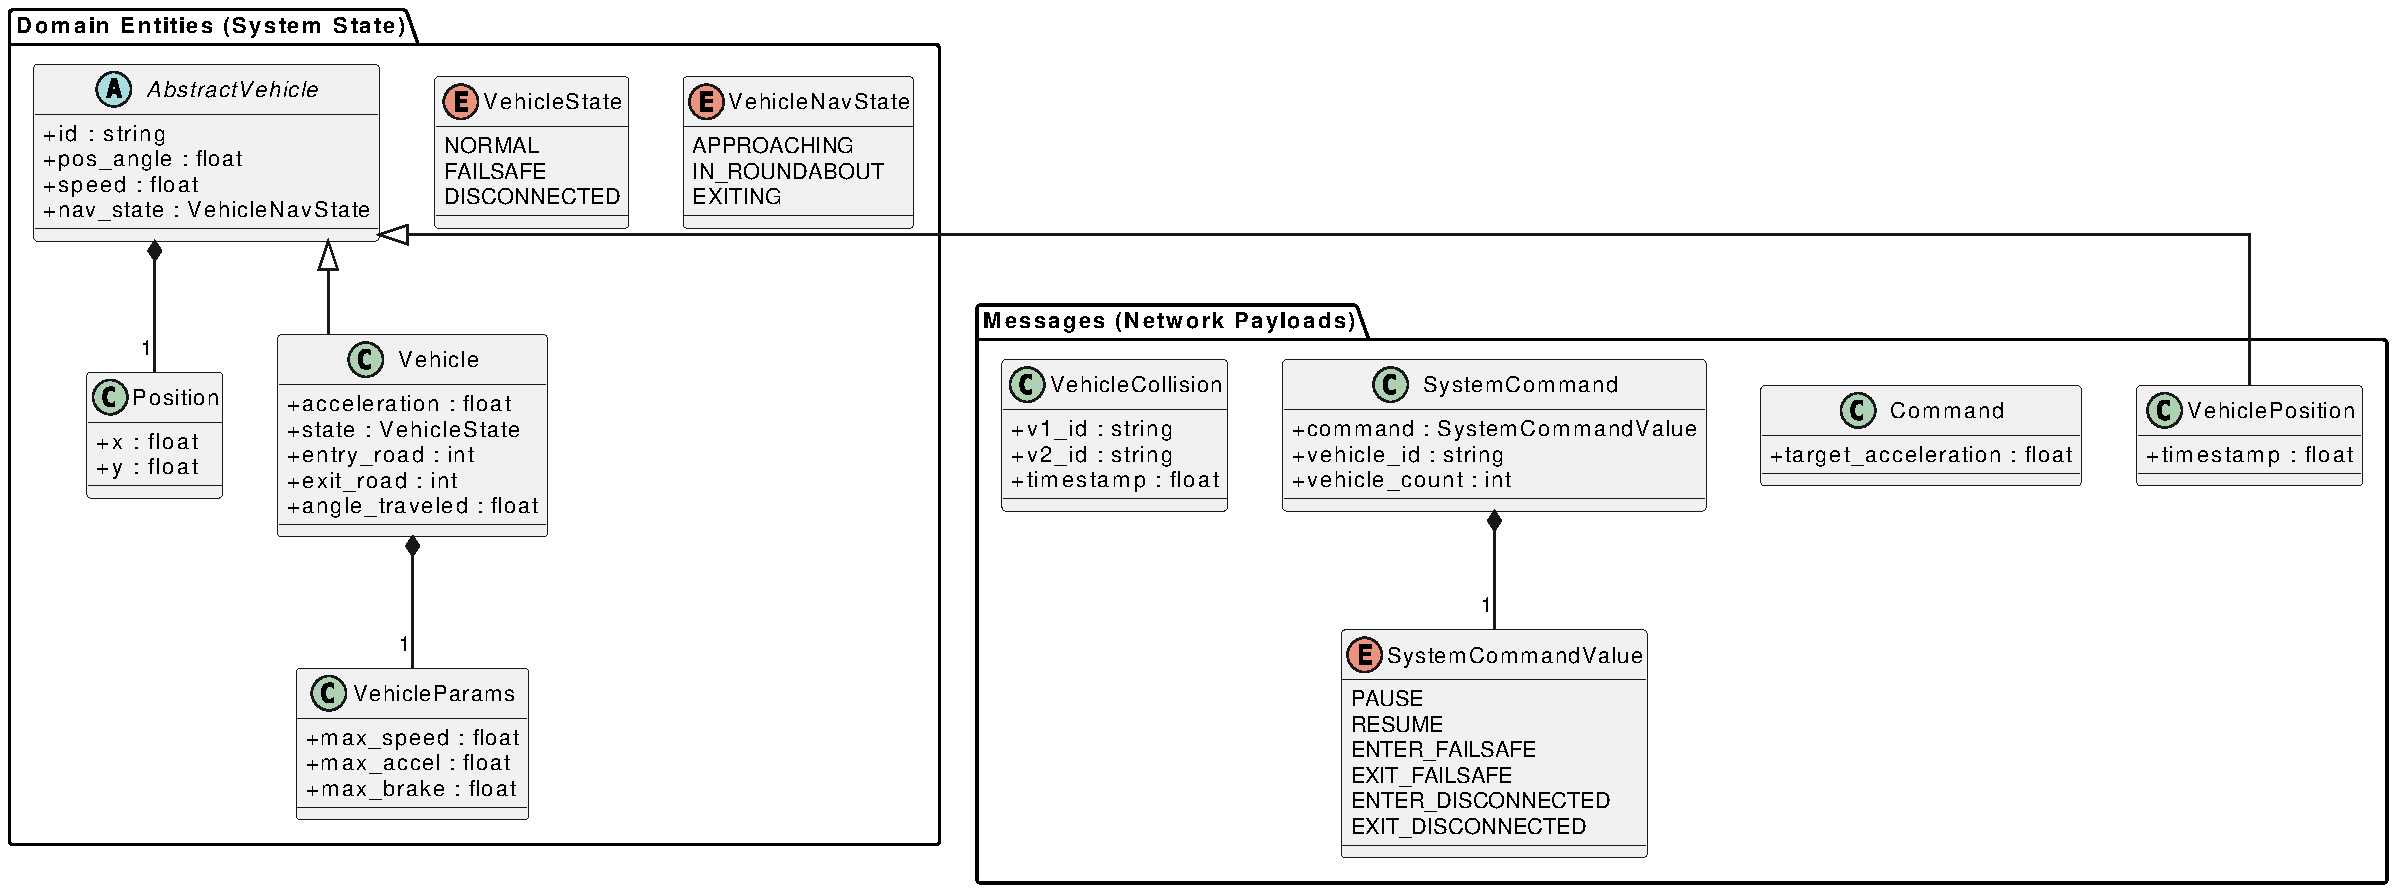
\includegraphics[width=\textwidth]{figures/class-diagram.pdf}
    \caption{Domain entities, as classes. Vehicles are used to represet the system's state, whereas other entities are transmitted as messages payloads.}
    \label{fig:class-diagram}
\end{figure}

\subsection{Interaction}\label{interaction}
All communications happen through the message broker, except the REST calls
between front-end and back-end of the visualizer web service.

Each \textbf{vehicle} periodically shares his data through the messages seen in
section \ref{arch:modelling}, with a constant rate:
\begin{itemize}
  \item its \textbf{telemetry}, if it's in a healthy state, for the controller;
  \item its \textbf{telemetry}, in any state, for simulation management and
  visualization purposes;
  \item its \textbf{local vision}, if it's in a healthy state, for the controller;
\end{itemize}

The \textbf{controller}, using the last vehicles' messages collected asynchronously,
periodically issues \textbf{commands} back to the responding vehicles.

The \textbf{simulation service} shares a collision when it's detected, on a dedicated
message channel --- read by the web service for visualization.

The \textbf{web server} displays vehicles, vehicles' states and controller's state, all
fetched periodically throught the broker. Moreover, upon receiving a system
command from the viewer, it sends the proper message (through the broker) to
vehicles or to the controller.

\begin{figure}
    \centering
    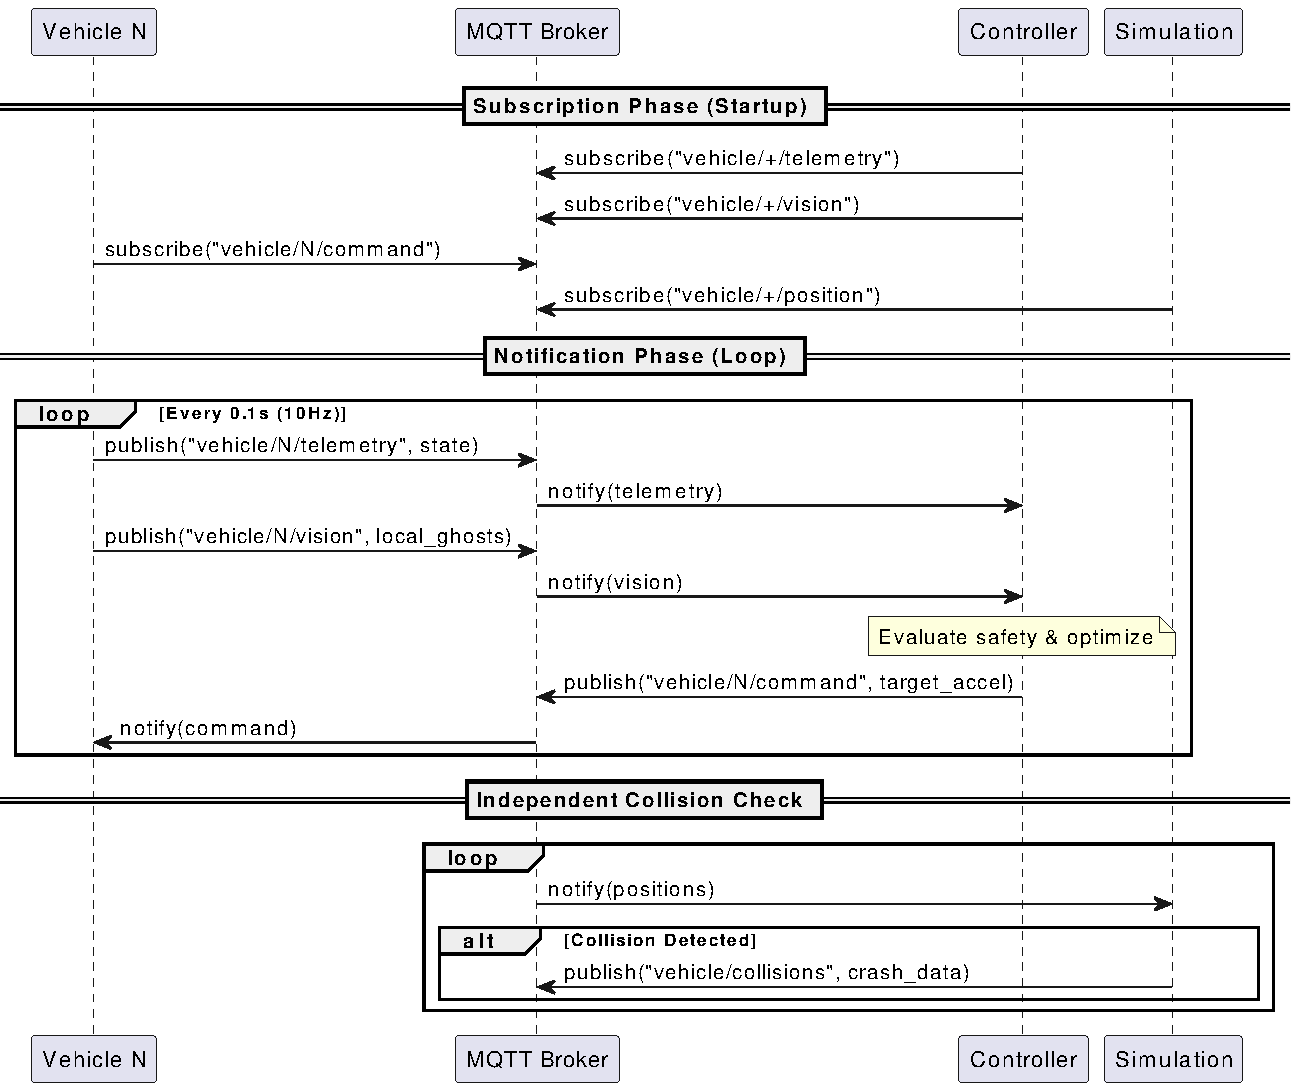
\includegraphics[width=\textwidth]{figures/sequence-diagram.pdf}
    \caption{Sequence of messages exchanged between the system components.}
    \label{fig:sequence-diagram}
\end{figure}

\subsection{Behaviour}\label{arch:behaviour}

In general, vehicles represent the ``truth'' of the system, since they are the
ones physically occupying a certain position and moving around, regardless of
the state of the network; to them, the controller is an external service which,
in normal conditions, they entrust to give them the most efficient, safe
driving command. Finally, the simulation and visualization services are mostly
mere observers --- with the visualizer that can forward system commands.
\\
\\
\subsubsection{Controller}\label{arch:behaviour_controller}
Starting from the \textbf{controller}, it continuously listens to vehicles'
messages (for their telemetry and their local vision) and, at the same time, it
periodically evaluates and issues commands, with a constant rate (currently 10
times per second).

Each received vehicle telemetry is saved together with a timestamp, in order to
only keep the most recent data and purge entries older than a certain threshold
(currently 0.5 seconds): these are called ``\textbf{active vehicles}''.
Moreover, before each evaluation cycle, the current position of each one is
estimated, by moving them by the distance they would have ridden, in their
current state, in the time interval since their communication: in this way, not
only are the positions presumably more accurate, but they also all refer to the
same instant.

The vehicles in their local vision, called ``\textbf{ghosts}'', are instead all
collected together, since they're just positions and can't be merged directly if
they represent the same one; to reduce their number, a more complex technique is
needed. Basically, each ghost is first moved to its predicted current position
(like for \textit{active vehicles}), then checked for collisions against the set
of each \textit{active} one: in case of a match, it's discarded, likely
referring to the same one; otherwise, it's saved as a distinct vehicle and will
also be checked for collisions with other \textit{ghosts}, to avoid to repeat
them.

Since entry and exit road aren't known for ghosts, additional precautions are
taken to further optimize the process. Entry isn't actually important: it's
obvious for an approaching car and irrelevant for an exiting one, whereas it
could be used to make predictions for one inside the roundabout (with the
assumption that they won't make more than one lap, from requirement 2.3, in
\ref{req:requirements}). The exit of a vehicle inside is instead very useful to
optimize the the entry of others. To grant the safety of the following
calculations, the worse options are assumed for a vehicle inside, and assigned
to each ghost: the last passed road is picked as both entry and exit.

Prediction of vehicles' current positions, ghosts merging and out-of-date
purging (for both vehicles and ghosts) are performed periodically before each
loop of command evaluation. It's important to remark that keeping the number of
vehicles (active plus ghosts) as low as possible is important for performance,
given the quadratic complexity of an evaluation and the fact that ghosts may
themselves be the squared number of total vehicles, if each one sees each other
one, possibly repeated if local vision messages are collected repeatedly. It
should also be noted that the more vehicles are disconnected from the network,
the less reliable this data will be, having more ``invisible'' nodes than those
contributing to the crowdsensing. Moreover, data can only be provided by
vehicles connected to the network (whether they're responding to commands or
driving in failsafe mode), but not by those which are completely disconnected
from the network.
\\
\\
The \textbf{evaluation} phase runs a sequence of checks for each active vehicle
$v_1$: in a single loop, it will be compared with each other active or ghost
vehicle $v_2$ --- only active vehicles will receive the resulting commands.

The general traffic principles for the controller are the following:
\begin{itemize}
  \item a vehicle, in any navigation state, should monitor the one in front to
  avoid to crash into it;
  \item approaching vehicles gain a priority level as soon as they get close 
  (within a threshold of a few meters) to
  the roundabout entry (basically FIFO, but not too rigid);
  \item vehicles inside generally have the priority;
  \item given the priority queue of approaching ones, a vehicle inside the
  roundabout should try to slow down and yield to an entering one, if it has a
  higher priority, but only if this can be done \textit{safely}. In the same
  way, an entering vehicle, even if it has higher priority on one coming from
  inside, shouldn't enter if this would put the one inside in a dangerous
  situation.
\end{itemize}

Controller's evaluations thus try to apply any possible optimization, as long as
these principles are always respected. To search for the highest safe
acceleration, for each $v_1$, the command is initially set to the maximum
possible value; each subsequent check against every $v_2$ can only lower it.
\\
\\
First of all, the \textbf{safety distance} for $v_1$ from $v_2$ in front is
defined, assuming they both started braking immediately, as the distance ridden
by $v_1$ before it stops minus the one ridden by $v_2$, plus the reaction
distance of $v_1$, plus an optional margin (so that the cars won't touch each
other once they will have stopped). Reaction distance, for $v_1$, is itself
defined as the distance ridden, with current speed and acceleration, in the time
before $v_1$ realizes it needs to brake and starts slowing down.
\[
  safe\_dist = (stop\_dist_{v_1} - stop\_dist_{v_2}) + react\_dist_{v_1} + safe\_margin
\]
To guarantee safety, one should use the maximum braking acceleration for $v_2$,
in case it has to brake for emergency, and a light deceleration for $v_1$, so
that it's able and ready to stop at any time with minimal wear on the mechanical
components. In this scenario, reaction time for the controller should be equal
to the data staling timer and the network timeout, because $v_1$ would have
ridden more distance in that interval, potentially getting to close to $v_2$; on
the other hand, a vehicle can have a negligible reaction time, when it controls
itself as a computer. Lastly, the safety margin can be set to a few meters, for
example the length of one car.

The main priority for the controller is to respect this constraint at all times:
$v_1$ can't accelerate if it doesn't have enough braking margin. Taking
advantage of the additional level of protection provided by the car's own
emergency braking system, the controller only sends a soft braking command when
the distance $dist$ between $v_1$ and $v_2$ is below $safe\_dist$: if the
message was to arrive to late to $v_1$, it would still start to brake on its own
when $dist$ gets below the lower safety distance calculated locally, i.e. using
a lower reaction time.
\\
\\
After having made sure that $v_1$ doesn't have to brake before a $v_2$ in front,
if it is close or inside the roundabout, the controller has to handle the most
critical points: the entrances.

When $v_1$ is about to enter, it will check for all vehicles already inside.
Those that will exit before its entrance can be safely ignored. For every other
$v_2$, it will be checked if $v_1$ can coordinate safely with it, i.e. if $v_1$
can either pass before or after while maintaining the proper safety distance: if
$v_1$ passes first, it shouldn't go so slower than $v_2$ such that $v_2$ will it
it soon after entering; if $v_1$ passes last, $v_1$ shouldn't go so fast that it
will hit $v_2$ after entering. The checks are performed for different values for
$v_1$'s acceleration, positive if possible, otherwise null (i.e. constant speed)
or negative (soft or hard braking) in the worst cases.

The $v_2$ inside itself is also under examination, in case it has to yield (to
someone with higher priority) or in case $v_1$ is close to the entrance. In both
situations, $v_2$ will try to facilitate the entrance of $v_1$ by slowing down
if needed, but only if it can be done safely --- otherwise, recall that who's
inside has the priority. Moreover, to safeguard the traffic flow, vehicles
inside never go below a certain speed threshold, unless the safety distance has
been violated, with respect to either the vehicle in front or the one about
to enter.

Additionally, vehicles in a \textit{failsafe} or \textit{disconnected} state are
given higher precedence at the intersection, i.e. a responding vehicle will try
to yield to them (again, safely). The first reason is to make them pass and get
rid of them as soon as possible, since they will drive slower and less
optimally. The second reason is to avoid \textbf{starvation} at all: vehicles in
failsafe mode are more ``timid'' and would risk to never be able to enter,
especially if there are only one or a few (refer to \ref{arch:behaviour_vehicle}
for vehicle logic).
\\
\\
Before an evaluation, in order to make the single loop of commands evaluations
more optimal, all vehicles (active plus ghosts) are \textbf{sorted} through a
simple heuristic, putting the ones with a higher priority first: exiting ones,
then inside ones, then approaching ones; approaching ones come first the closer
they are to the center, while exiting ones come first the further they are;
inside ones are picked in clock-wise order.

In this way, before evaluating for $v_1$, the speed of a $v_2$ in front is
always already known, since it will have been processed first: this makes the
safety distance estimates more correct. The only exception, not taken into
consideration, regards the ``junction point'' for the ones inside: since they
are taken in clock-wise order starting from a random point, the first picked
vehicle will be evaluated before the one in front of it. Moreover, inside
vehicles come before approaching ones because they generally have the priority.
Once in the exiting state, instead, they have already passed the intersection
and don't have many possible conflict, but should only care about who's in
front.
\\
\\
Knowing the controller's functioning mechanism, it's now possible to see that
its complexity is approximately quadratic in the number of total vehicles.
Deeper studies on a real scenario would be required to understand if the
evaluation frequency could be increased. Improved estimations would in fact come
at a higher computational cost, possibly even made worse by an higher number of
vehicle nodes; however, a server of modest dimensions may be able to handle
them.

\subsubsection{Vehicle}\label{arch:behaviour_vehicle}
Each vehicle repeatedly (currently 10 times per second) runs a procedure to take
a decision (on the new acceleration to apply) and to apply it, proceeding then
to update its own position by physically moving according to its speed,
direction and destination. In parallel, it also listens for commands from
controller and web server and publishes its data.

An actuation loop starts with a local check an \textbf{emergency} command; if
it's not needed, the vehicle uses the last received controller's command if it's
available and not too old, otherwise runs its own evaluation logic: it thus
assumes that there's a network problem and goes in \textbf{failsafe} mode. After
having taken and applied the decision, it will try in all cases to share its
updated position with the controller: if the connection had been lost, this is
used as a heartbeat, to try to re-establish it; if it's driving in failsafe mode
for necessity, it will still update the controller so that it can give better
commands to the others, even if the vehicle itself won't execute the received
ones.
\\
\\
The checks performed in both \textbf{emergency} and \textbf{failsafe}
evauluations are very similar to the controller's ones
(\ref{arch:behaviour_controller}).

The \textbf{emergency} evaluation only does checks about safety distance, using
hard brakes: in the tail-gating case (against a vehicle in the same navigation
state) and near the intersection points, whether it's the one approaching or the
one inside.

The \textbf{failsafe} evaluation, with respect to the controller's one, has the
main differences of imposing a lower maximum speed and of making the vehicle
always stop before entering the roundabout. For the intersections, if it's
entering the logic will be similar to the controller one's, whereas, if it's
inside, it won't do anything to try to slow down, do optimizations or yield. In
fact, regarding the security, the \textit{emergency} mechanism already takes
care of all cases of emergency brakes, while, regarding the optimization, the
vehicle partly lacks information on the others in order to make the best
decisions, partly assumes the others will follow the traffic rules: whether
they're follow the controller's commands or their owns, each logic still aims to
only do safe moves.

\subsubsection{Simulation}
The simulation service only takes care of identifying and publishing any
collisions, calculated by looking for pairs of overlapping cars.

The state of the simulation system is actually kept be the vehicles, each
knowing (and publishing) its position.

The number of vehicles remains always the same; when one gets far enough from
the roundabout, it respawns with new random start and destination.

\subsubsection{Web-viewer}
The web-viewer service makes it possible for a spectator user to visualize and
interact with the system.

The service listens to and saves all vehicles states, controller's state and
simulation's collisions.

It then exposes API endpoints to read its state and to post controls, to one or
more vehicles, to pause and resume the simulation or to go into failsafe or
disconnected mode.

\begin{figure}
    \centering
    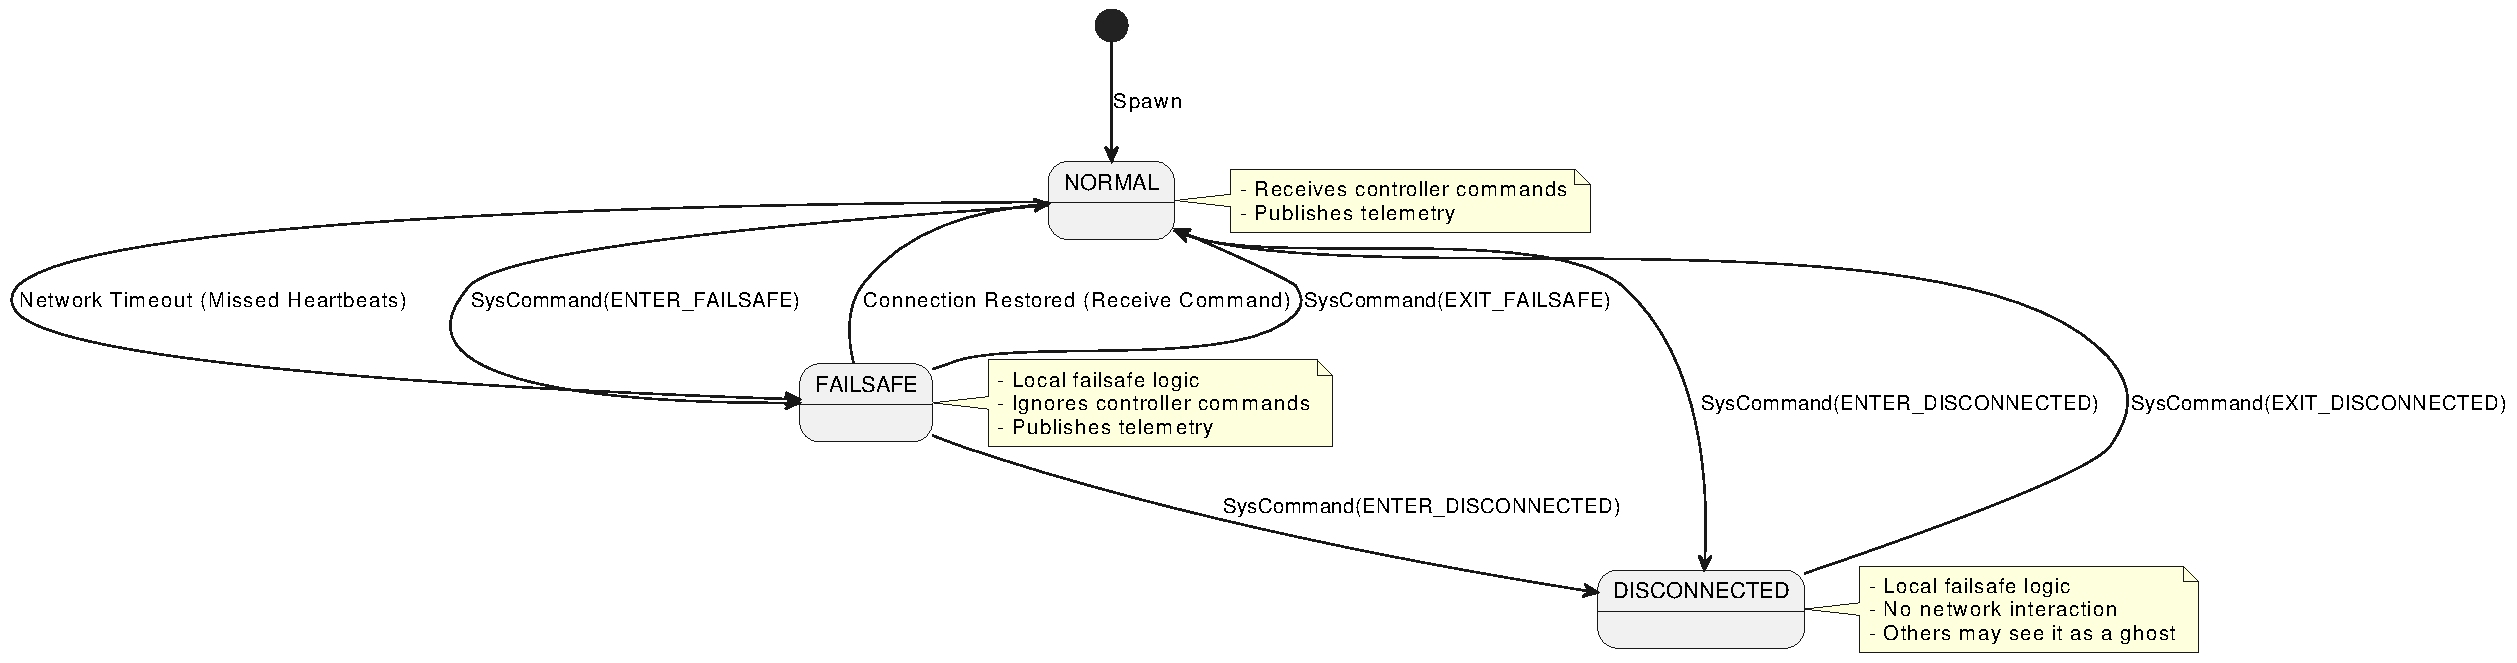
\includegraphics[width=\textwidth]{figures/state-diagram-vehicle.pdf}
    \caption{Vehicle states and the transitions between them.}
    \label{fig:vehicle-state-diagram}
\end{figure}

\subsection{Data and Consistency Issues}\label{data-and-consistency-issues}
No data needs to be stored, since everything is used almost immediately and old
data is soon considered stale and unusable; on the contrary, for the current
tasks, a database would only introduce latency, which would be a problem.
Therefore, data is currently only being stored in in-memory dictionaries.

A database may only be useful as an additional service, subscribing to the same
message topics in order to collect the system's data for later analysis and
debugging (for example, even in case of accidents).
\\
\\
The system uses \textbf{eventual consistency}; after all, every component's view
is always behind the physical reality, only known by the cars themselves, and a
network disconnection will increase the delay. Nonetheless, vehicles
continuously publish their data, so that a listener will sooner or later fetch
the latest state.

Additionally, the controller tries to improve the consistency of its state with
the real one through the prediction mechanism (\ref{arch:behaviour_controller}).

\subsection{Fault-Tolerance}\label{fault-tolerance}
Accepting the possibility of errors is one of the main concerns of the project;
after all, this is a simulation of vehicles, meaning that they are constantly
moving and can't afford to stop and wait for the signal to come back or the
problems to be fixed. So, when messages don't travel successfully between the
controller and a vehicle, they are simply \textbf{ignored}: each vehicle also
has its own logic (\ref{arch:behaviour_vehicle}), to be able to somehow proceed
safely even without the controller's commands; the controller will try it best
to provide optimal commands to the remaining healthy ones
(\ref{arch:behaviour_controller}).

The vehicles' failsafe and emergency modes hence contribute to increase the
\textbf{reliability} of the system (\ref{req:distr_dependability}). Unexpected
events may always occur, especially if many vehicles are disconnected from the
network and, consequently, the controller can't have fully reliable data on
them. Moreover, in the real world, there could always be other obstacles on the
road, objects, pedestrian, etc.

\textbf{Timeouts} are fundamental to mark vehicles' and controller's data as old
and no longer usable. Messages between the two components are used as
\textbf{heart-beats}: a vehicle is considered healthy as long as it keeps
communicating forth and back and, even if it loses the connection, it will
return to a normal state as soon as it will be able to share its position and
receive a command from the controller.
\\
\\
Availability and fault tolerance improvements, however, haven't been considered
for the \textbf{controller}. One possibility would be to deploy more controller
nodes to use as \textit{master-slave replication}: one is elected as the working
one, while the others only follow to keep their state up to date; in case of
failure, a replica will become the new master. This approach would avoid to add
latency, since the replicas don't need to communicate in normal conditions.

\subsection{Availability}\label{availability}


\subsection{Security}\label{security}
Security hasn't been considered deeply in the development, for lack of time,
despite the observations in \ref{req:distr_security}.

According to the current design, the system has already been thought to prevent
accidents due to wrong commands, thanks to the cars' \textit{local vision} and
the \textit{failsafe} and \textit{emergency mode} that can take control in case
of need; however, an overflooding of inexisting cars' positions could still lead
the controller to block the entire system.
\\
\\
In this implementation, the docker network is assumed to be secure; future
improvements may require authentication through TLS for message exchange and
provide a unique cryptographic key to each vehicle. For separation of concerns,
the broker may also verify authorization through Access Control Lists, where
each role is only authorized to publish on certain message topics:
\begin{itemize}
  \item \textit{Vehicle N}: can only share its own data and subscribe to
  commands directed to it;
  \item \textit{Controller}: can subscribe to all telemetry and publish commands
  for all;
  \item \textit{Admin}: can publish system commands.
\end{itemize}
